% -*- TeX-engine: default; -*-
\documentclass[10pt,sigconf]{acmart}
\usepackage[font=footnotesize]{subcaption}
\usepackage[utf8]{inputenc}
\usepackage[T1]{fontenc}
\usepackage{url}
\usepackage{booktabs}
\usepackage{xcolor}
\usepackage{enumitem}
\usepackage{algorithm}
\usepackage[noend]{algpseudocode}

\setcopyright{rightsretained}
\acmYear{2018}
\copyrightyear{2018}
\acmConference[CoNEXT'18]{ACM CoNEXT 2018}{December 2018}{Heraklion/Crete, Greece}

\begin{document}
\title{The eXpress Data Path: Programmable Packet Processing for the Linux Kernel}
\author{Toke Høiland-Jørgensen}
\affiliation{%
  \institution{Karlstad University}
  \country{Sweden}}
\email{toke.hoiland-jorgensen@kau.se}

\author{Jesper Dangaard Brouer}
\affiliation{%
  \institution{Red Hat}
  \country{Denmark}}
\email{brouer@redhat.com}

% \renewcommand{\shortauthors}{T. Høiland-Jørgensen et al.}
\renewcommand{\shorttitle}{The eXpress Data Path}
\captionsetup{font+=small}



\begin{abstract}
  Programmable packet processing in software has become increasingly popular, as
  increases in computational power has made it possible to run custom
  programmable pipelines at high speeds. This is generally implemented by
  so-called kernel bypass techniques, where a userspace application takes
  complete control of the networking hardware to avoid expensive context
  switches between kernel and user space.

  However, this approach makes high-speed packet processing an all-or-nothing
  proposition, where the processing application has to handle all network
  traffic, reinventing a lot of functionality already present in the kernel.
  Interoperability with other applications is also difficult, requiring
  cumbersome re-injection of packets into the kernel.

  In this paper, we present an alternative approach to programmable packet
  processing, where the kernel provides a safe execution environment for custom
  packet processing applications, executed directly in the context of the kernel
  device driver. This system, called the eXpress Data Path (XDP), is part of the
  mainline Linux kernel, and has been gradually expanded over the last several
  releases. We describe the design of the system and how it integrates with the
  rest of the kernel. Through a range of real-world examples we illustrate the
  flexibility of this model and how it can be used to implement a wide range of
  applications with performance measure in tens of millions of packets per
  second.
\end{abstract}

% TODO: Add ccsxml tags and update keywords

\keywords{XDP, Programmable Networking}
\maketitle

\section{Introduction}
\label{sec:introduction}
High-performance packet processing in software has very tight bounds on the time
spent processing each packet ($\simeq67$~ns per packet at 10 Gbps). Network
stacks in general purpose operating systems typically perform way too many
operations per packet to be able to keep up with this packet rate, which has led
to the introduction of special-purpose networking toolkits for software packet
processing, such as DPDK and Netmap. However, these toolkits have the drawback
that they are difficult to integrate with the existing networking stack, leading
to the need to re-implement large parts of the stack.

We present an alternative to previous approaches: A novel way to integrate
programmable packet processing directly into the networking stack in a
cooperative way, making it possible to perform high-speed packet processing that
integrates seamlessly with existing applications. This framework, called the
eXpress Data Path (XDP), works by defining a limited execution environment based
on an extended version of the Berkeley Packet Filter bytecode language, which
allows verified programs to run directly in kernel context before the normal
packet processing in the networking stack.

This makes it possible to implement applications that previously required their
own appliance, such as DDOS protection and load balancing, directly on
application servers. It also allows a hybrid approach, where certain fast path
processing is offloaded to XDP while retaining normal network stack processing
for other packets. This allows for exceptionally high throughput and low latency
processing without sacrificing flexibility.

We present the design of XDP and its capabilities and integration with the Linux
kernel. We then present a performance evaluation that consists of
micro-benchmarks showing packet processing scaling beyond 20 Mpps on a single
core as well as two real-world use cases: inline DDOS protection and layer-3
packet forwarding.

\section{Related work}
\label{sec:related-work}
\section{The design of XDP}
\label{sec:design}
XDP is designed to integrate with the Linux networking stack, enhancing it with
high-performance programmable hooks in strategic places. This makes it possible
to take advantage of the extensive and robust features of the operating system,
while adding custom packet processing as required. For this reason, XDP should
not be seen as a monolithic system one injects a single program into, but rather
a composition of individual parts that operate in concert to achieve the desired
outcome.

\begin{figure*}[t]
\centering
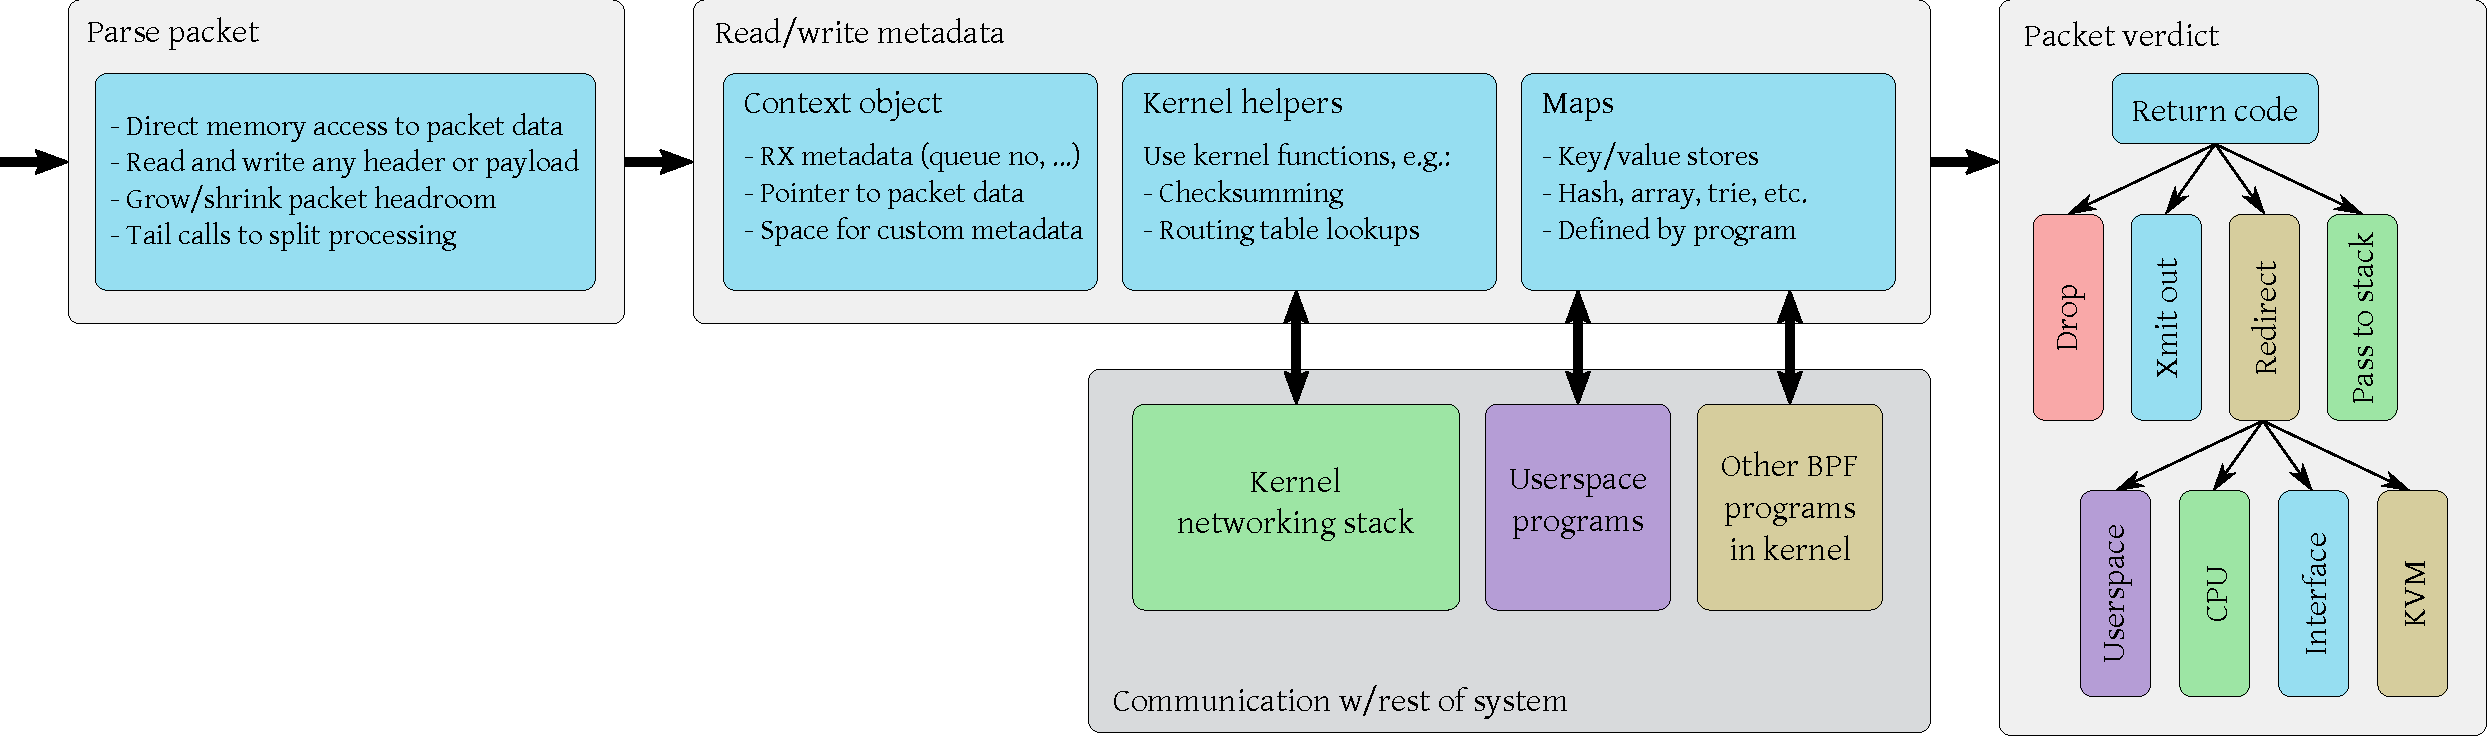
\includegraphics[width=\linewidth]{figures/xdp-execution-diagram.pdf}
\caption{\label{fig:xdp-execution} Execution diagram of a typical XDP program.
  When a packet arrives, the program starts by parsing packet headers to extract
  the information it will react on. Based on this, combined with information
  from one or more of the metadata facilities, a packet can be rewritten and a
  final verdict for the packet determined. The program can alternate between
  packet parsing, metadata lookup and rewriting, all of which are optional. The
  final verdict is given in the form of a program return code.}
\end{figure*}

This section describes the various parts of the XDP system and how they fit
together. We begin with a high-level overview of the XDP programming model and
how various features of the kernel combine to form a powerful programmable data
plane. Following this, we look in detail at the extended BSD Packer Filter
(eBPF) virtual machine providing the execution model, and the in-kernel verifier
that ensures the safety of loaded eBPF programs.

\subsection{The XDP programming model}
\label{sec:prog-model}
The XDP system enables high-performance packet processing integrated tightly
with the rest of the Linux networking stack. This makes XDP unique compared to
other high-performance software packet processing frameworks, because it makes
it possible to selectively leverage features already implemented in Linux, while
writing custom programs to perform application-dependent processing, or to
accelerate certain parts of the data path. This section gives a conceptual
overview of the XDP programming model, explaining how the different parts fit
together.

An XDP program is run in the eBPF virtual machine and is entirely event driven.
The program is executed directly in context of the device driver, without
context switching to userspace. The program is executed at the earliest possible
moment after a packet is received from the hardware, before the kernel allocates
any data structures or performs any parsing of packet data. This allows for high
performance, but the program has to parse raw packet data itself.

Figure~\ref{fig:xdp-execution} gives a conceptual overview of the execution of a
typical XDP program. The program starts its execution with access to a pointer
to a context object. This object contains the buffer of the raw packet data,
along with metadata fields describing which interface and receive queue the
packet came in on, etc. The program can read and write any parts of the packet
data buffer, including expanding or shrinking the packet to add or remove
headers. It can also pass control to a different XDP program, through a
so-called \emph{tail call}, which executes the target program and never returns
to the caller, thus splitting processing into logical sub-units (based on, say,
IP header version). The context object also contains a pointer to a special
memory area is available for XDP to store arbitrary metadata that will be
available to other XDP programs, as well as to other parts of the kernel and
userspace (under certain circumstances).

Similar to a regular userspace program, an XDP program ends its execution with a
return code, instructing the kernel what to do with the packet. There are three
simple return codes which either drop the packet, immediately re-transmit it out
the same network interface, or allow the packet to be processed by the kernel
networking stack. In addition to these simple actions, the XDP program can
\emph{redirect} the packet, which controls its further processing. Redirecting
can be used to transmit the packet out a different network interface, to pass it
to a different CPU to further processing, to pass it to a virtual machine
running on the host, or to pass it directly to a special userspace socket
without copying.

\begin{figure}[t]
\centering
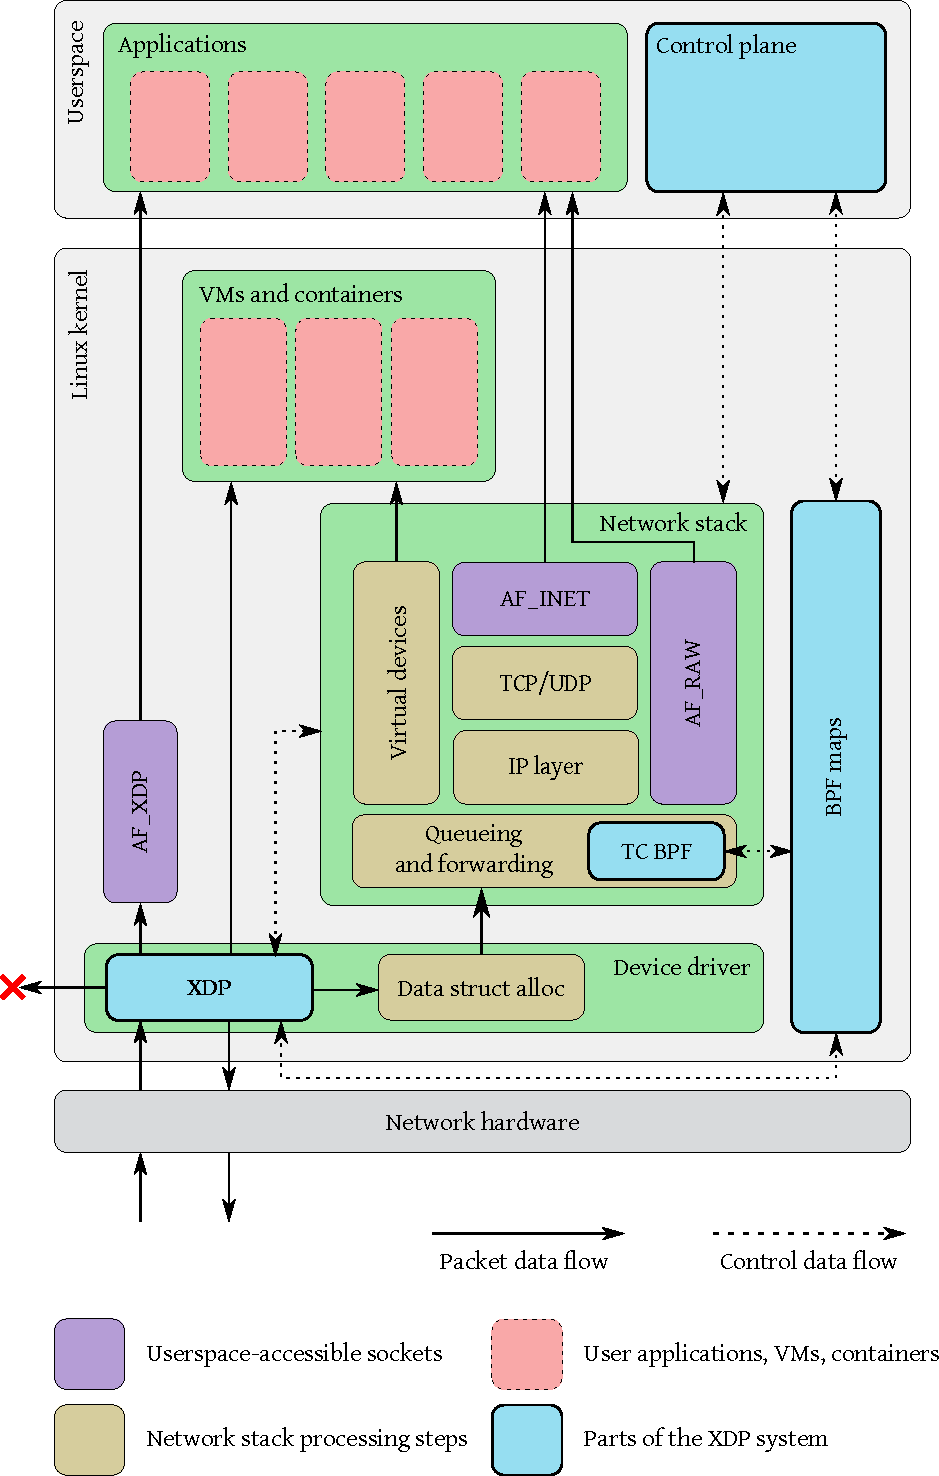
\includegraphics[width=\linewidth]{figures/kernel-diagram.pdf}
\caption{\label{fig:xdp-kernel} Diagram of how XDP integrates into the Linux
  kernel network receive path.}
\end{figure}

During its execution, and XDP program also has access to kernel facilities that
provide helper functions and additional metadata. Figure~\ref{fig:xdp-kernel}
shows a diagram of how XDP integrates into the full system. The XDP hook in the
driver is the first thing that is executed after a packet is received from the
network hardware. This program can control how further packet processing is
performed as described above (solid lines). In addition to this, the facilities
given to interact with the kernel allow the XDP program to gather additional
metadata (dotted lines), through helper functions and maps. Helper functions are
callbacks implemented in the kernel that an XDP program can call to make use of
kernel functionality in its processing. These helpers range serve various
purposes, ranging from simple checksum computation and hashing, to full access
to the kernel routing table. New helpers are actively been added by the kernel
development community in response to user requests, continuously expanding the
functionality that XDP programs don't have to re-implement themselves.

Maps are key/value stores that are defined by the user before loading an XDP
program, and can be referred to from within the eBPF code. Maps are shared, both
between different eBPF programs running at various places in the kernel, as well
as between eBPF and userspace. The map types include generic hash maps, arrays
and radix trees, as well as specialised types containing pointers to eBPF
programs, or even recursive pointers to other maps. Maps serve several purposes:
they are a persistent data store between invocations of the same eBPF program; a
global coordination tool, where eBPF programs in one part of the kernel can
update state that changes the behaviour in another; and a communication
mechanism between userspace programs and the kernel eBPF programs, similar to
the communication between control plane and data plane in other programmable
package processing frameworks. These different communication paths are marked
with dotted lines in Figure~\ref{fig:xdp-kernel}.

Another piece of the XDP picture is the ability to run eBPF programs in other
parts of the kernel. These include packet processing in the Traffic Control (TC)
subsystem, where eBPF programs can filter packets after they have been parsed by
the kernel, or before they are passed to the hardware from applications. This is
marked as ``TC BPF'' in the figure. In addition, eBPF programs can be attached
to various places in the kernel that are unrelated to networking (not shown on
the figure). These include \emph{cgroups}, which control resource usage for
groups of processes (used for implementing containers on Linux, for instance),
as well the \emph{tracepoint} and \emph{kprobe} introspection subsystems which
allow attaching eBPF programs to arbitrary kernel functions. Because all eBPF
programs can share the same set of maps, this makes it possible for XDP programs
to react to arbitrary events in the kernel, for instance by dropping packets if
processing load increases. Because of this integration, the XDP programming
model is considerably more powerful than just the XDP programs itself.

A final important feature of the XDP system is the ability to dynamically load
eBPF programs. Because the kernel manages the life cycle of all eBPF programs,
they can be dynamically loaded and reloaded at runtime. Combined with dynamic
dispatch to other programs using tail calls, this makes it possible to limit the
amount of processing actually performed on packets. A processing pipeline can
simply split its processing into separate XDP programs and dynamically load and
unload them as features are enabled or disabled through control plane
configuration. This also makes it possible to dynamically compile programs with
hard-coded values derived from configuration, avoiding expensive data structure
lookups for common tasks.

The various pieces of the XDP system outlined above combine to form a powerful
programmable data plane, with integration into the Linux kernel aiding
deployment on existing systems. The following sections describe the eBPF virtual
machine itself, and the verifier that ensures that loaded programs are safe to
run in kernel space.

\subsection{The eBPF virtual machine}
\label{sec:bpf-vm}
The eBPF virtual machine is an evolution of the original BSD packet filter (BPF)
\cite{mccanne_bsd_1993} which has seen extensive use in various packet filtering
applications over the last decades. BPF uses a register-based virtual machine to
describe filtering actions. This virtual machine has two 32-bit registers and
understands 22 different instructions. This makes BPF well-suited for packet
filtering operations, but limited as a general purpose virtual machine. eBPF
extends the original BPF virtual machine to allow full general purpose execution
and efficient just-in-time (JIT) compilation into native machine code. Support
for compiling (restricted) C code into eBPF is included in the LLVM compiler
suite

The code running in the virtual machine is executed directly in the kernel
address space, which makes eBPF useful for a wide variety of tasks in the Linux
kernel. The verifier (described in the next section) ensures that user-supplied
programs cannot harm the running kernel, which enables a wide array of
integrations between the running kernel and the XDP system.

The eBPF modifies the BPF virtual machine as follows:

\begin{table}[htbp]
\caption{\label{tbl:reg-map}
eBPF to x86\_64 register mapping.}
\centering
\begin{tabular}{ll}
\toprule
eBPF & x86\_64\\
\midrule
R0 & rax\\
R1 & rdi\\
R2 & rsi\\
R3 & rdx\\
R4 & rcx\\
R5 & r8\\
R6 & rbx\\
R7 & r13\\
R8 & r14\\
R9 & r15\\
R10 & rbp\\
\bottomrule
\end{tabular}
\end{table}


\begin{itemize}
\item The number of registers is increased to eleven, and register widths are
increased to 64 bits, with 32-bit sub-registers accessible through certain
instructions to provide compatibility with classic BPF programs. The 64-bit
registers map one-to-one to hardware registers on all 64-bit architectures
supported by the kernel, which eases JIT compilation. For instance, the x86\_64
JIT compiler uses the mapping shown in Table \ref{tbl:reg-map}.

\item eBPF adds a \emph{call} instruction for function calls, and adopts the same calling
convention as the C language conventions used on the architectures supported
by the kernel. Along with the register mapping mentioned above, this makes it
possible to map a BPF call instruction to a single native call instruction,
enabling function calls to native kernel functions with close to zero
overhead. This facility is used by eBPF to support helpers that eBPF programs
can call to interact with the kernel while processing.

The eBPF calling convention is as follows:
\begin{itemize}
\item \texttt{R0} contains the function return value
\item \texttt{R1}-\texttt{R5} contains function arguments
\item \texttt{R6}-\texttt{R9} are callee saved registers that will be preserved across the call
\item \texttt{R10} is a read-only frame pointer to the beginning of the eBPF stack space
\end{itemize}
\end{itemize}


A BPF program starts its execution with \texttt{R1} containing a pointer to a \emph{context}
object, the contents of which varies with the type of program. For XDP, this
points to a structure that allows the BPF program to access the packet data
itself, as well as various items of metadata, including space for arbitrary data
that is carried along with the packet and is accessible by other BPF programs
that operate on the packet at later stages of processing.


\subsection{The eBPF program verifier}
\label{sec:bpf-verifier}
As mentioned in the previous section, eBPF code runs directly in the kernel
address space, which means that it theoretically has full access to the running
kernel and can either crash or compromise this. To avoid this unpleasant
situation, the kernel enforces a single entry point for loading all BPF programs
(through the \texttt{bpf()} system call). When loading a BPF program it is first
analysed by the in-kernel \emph{BPF verifier}, which ensures that the program
performs no actions that are unsafe (such as reading arbitrary memory), and that
the program will terminate by disallowing loops and limiting the maximum program
size. The verifier works by first building a directed acyclic graph (DAG) of the
control flow of the program. This DAG is then verified as follows:

First, the verifier performs a depth-first search on the DAG to ensure it
contains no loops (no backwards jumps) and that it contains no unsupported or
unreachable instructions. Then, in a second pass, the verifier walks all
possible paths of the DAG while tracking the state of all registers. The purpose
of this second pass is to ensure that the program performs only safe memory
accesses, and that any helper functions are called with the right argument
types. This is ensured by rejecting programs that perform load or call
instructions with invalid arguments. Argument validity is determined by tracking
the state of all registers and stack variables through the execution of the
program, as explained in the following.

\subsubsection{Register state tracking}
\label{sec:reg-state}
To track data access, the verifier assigns five state variables to each
register, listed in Table \ref{tbl:vrf-state-vars}, with the possible types listed in
Table \ref{tbl:reg-types}. The fixed offset is used to track the result of pointer
arithmetic with fixed values, while the ranges and \emph{tnum} are used to track
variable offsets of pointers, as well as the ranges of scalar variables.

At the beginning of the program, \texttt{R1} contains a pointer to the execution
context, and its type is a \texttt{CTX} pointer; \texttt{R10} is a \texttt{STACK}
pointer, and all other registers are \texttt{NOT\_INIT}. At each execution step,
register states are updated based on the operations performed by the program.
When a new value is stored to a register, it inherits the state variables of the
source of the value. Arithmetic operations on scalar values will affect the
value of the \emph{tnum} state variable, which tracks which bits in a register
are known, and their value. The \emph{tnum} is a pair of \emph{mask}, which
contains the bits whose value is unknown, and a \emph{value} which contains the
bits that are known to be set to 1. Load operations set these, for instance
loading a byte from memory will result in the top 56 bits being known to be
zero, and the bottom 8 bits to be unknown. Arithmetic updates these values
according to their operation.

Branches in the instruction tree will update the register state according to the
logical operation contained in the branch. For example, a comparison "\texttt{R1
  > 10}" compare will set the maximum value of \texttt{R1} to 10 in one branch,
and the minimum value to 11 in the other. If a comparison is performed with a
scalar value rather than a constant, the knowledge of which bits are set is used
to compute the ranges for the branches (using the minimum and maximum possible
values of unknown bits as appropriate). Finally, a branch that checks whether
register with a \texttt{MAP\_VALUE\_OR\_NULL} pointer is different from
\texttt{NULL} will turn that register into a pointer with type
\texttt{MAP\_VALUE} in the \emph{true} branch, which makes it possible to
derefence the pointer.

Using the information contained in the state variables, it is possible for the
verifier to predict the ranges of memory that it is possible for each load
instruction to access. It uses this information to ensure that only safe memory
accesses are performed. For pointers to context objects, the execution context
of the eBPF program indicates allowed memory offsets for their context objects
through a callback performed by the verifier. For map values, the map definition
defines the size of the values, which is used to bound the allowed memory
accesses. For pointers to stack values, only ranges previously stored on the
stack are valid. And finally, for pointers to packet data, only ranges known to
be less than the packet length (by appropriate compares against the packet end
pointer) are allowed. Any eBPF program that makes memory accesses that the
verifier cannot prove are safe are simply rejected at load time. The verifier
also uses the range information to enforce aligned memory accesses.

When pointers are copied to other registers, a bounds check on one copy can be
used to infer the valid ranges of the other copies, even after the copy
occurred. The \emph{id} state variable is used for this purpose for packet access and
map value pointers. For packet access, all pointers with the same variable
range will have the same \emph{id}, even if their fixed offset differs. Thus, a range
check on one copy will mark the same range (minus any differences in fixed
offsets) as valid in the other copies. Similarly, for pointers to map values,
all copies of a pointer returned from the same map lookup share their \emph{id}, and
a check against NULL will be valid for all of them.

\begin{table}[htbp]
\caption{\label{tbl:vrf-state-vars}
eBPF verifier state variables}
\centering
\begin{tabular}{ll}
\toprule
Variable & Contains\\
\midrule
\texttt{type} & One of the types in Table \ref{tbl:reg-types}\\
\texttt{id} & ID for tracking copies of same variable\\
\texttt{fixed\_offset} & Pointer offset (after arithmetic)\\
\texttt{range\_unsigned} & Min and max values (unsigned)\\
\texttt{range\_signed} & Min and max values (signed)\\
\texttt{tnum} & Mask and value of known bits\\
\bottomrule
\end{tabular}
\end{table}

\begin{table}[htbp]
\caption{\label{tbl:reg-types}
eBPF verifier type annotations. The last column indicates whether pointer arithmetic is allowed for this type of pointer.}
\centering
\begin{tabular}{lll}
\toprule
\multicolumn{3}{c}{\textbf{Non-pointer types}} \\
Name & Meaning \\
\midrule
\texttt{NOT\_INIT}            & Not initialised         \\
\texttt{SCALAR\_VALUE}        & Any numerical value       \\
\midrule
\multicolumn{3}{c}{\textbf{Pointer types}} \\
Name & Pointing to & Arithm\\
\midrule
\texttt{CTX}                  & Context              & Yes \\
\texttt{MAP}                  & BPF map              & No  \\
\texttt{MAP\_VALUE}           & Value in map         & Yes \\
\texttt{MAP\_VALUE\_OR\_NULL} & Value in map or NULL & No  \\
\texttt{STACK}                & Stack frame          & Yes \\
\texttt{PACKET}               & Packet data start    & Yes \\
\texttt{PACKET\_END}          & Packet data end      & No  \\
\bottomrule
\end{tabular}
\end{table}
\section{Performance evaluation}
\label{sec:perf-eval}
\subsection{Micro-benchmarks}
\label{sec:org72788e2}
\subsection{Comparison with DPDK/netmap}
\label{sec:org7f03063}
\section{Real-world use cases}
\label{sec:org60dd487}
\subsection{DDOS mitigation}
\label{sec:org5f83e1d}
\subsection{Packet forwarding layer 2/3}
\label{sec:org3681460}
\begin{itemize}
\item Helper functions into bridging / routing code
\item Layer 2 also useful for VMs
\end{itemize}
\subsection{Load-balancer}
\label{sec:org685e28c}
\begin{itemize}
\item \texttt{XDP\_TX}
\item \texttt{XDP\_REDIRECT} to CPU/VM
\end{itemize}
\section{Conclusions}
\label{sec:conclusion}





\bibliographystyle{ACM-Reference-Format}
\bibliography{xdp}

\end{document}
